%!TEX root = ./main.tex
%
% This file is part of the i10 thesis template developed and used by the
% Media Computing Group at RWTH Aachen University.
% The current version of this template can be obtained at
% <http://www.media.informatik.rwth-aachen.de/karrer.html>.

\chapter{Summary and Future Work}
\label{summaryandfuturework}

\section{Summary and Contributions}
\label{summaryandfuturework.summary}
We presented a 2D textile touchpad for eyes free interaction capable of detecting up to eight free-form gestures with 84.5\% reliability on average. The touchpad is composed of textile materials that are flexible, lightweight, breathable, and washable. It is composed of two layers of fabric with conductive yarn sandwiching a space made of 3mm foam. The touchpad is based on the simple principles of resistive touch technology which has some advantages over capacitive technology when it comes to wearable touch sensing, namely neglecting the noise of the human body. Most of the prototypes which use capacitive touch are rather limited in the gestures they can detect due tho the noise of the human body. Our prototype only yields a touch if the layers are physically connected. The limitations of our approach are low resolution and the need of a certain amount of force to connect the conductive layers. We evaluated the robustness of the textile touchpad as a wearable sensor by testing gesture recognition rate and noise generated under three extreme conditions: softness, curvature, and friction. We found that, despite the low resolution of 14 by 14, we are able to detect more complex unistroke gestures.
\\ \\
We described how we built our prototype with low cost materials. We explained step by step how to attach the pinstripe fabric layers to the spacing material, such that everyone is able to rebuild it in short time. The necessary code is linked in the chapter~\ref{appendix}. Our prototype is easy scalable and is only limited in the number of pins of the used microcontroller. Although we made our prototypes equilateral, it is simply possible to give it any rectangular size. 
\\
Furthermore we explained the software for our sensor to detect simple unistroke mark-based gestures using our own recognizer. The sensor is able to recognize more complex unistroke free-form gestures using the 1\$ recognizer. This is the first full textile touchpad being able to do that consistently. We tested the prototype under multiple conditions to evaluate the physical limitations of the sensor. We implemented the recognition with an threshold of 3 milliseconds such that the impact of contact loss is lower. Such a contact loss is caused by too little pressure or slipping of the prototypes touch sensing area due to the curvature illustrated in figure~\ref{fig:curvatureillustration}. We found that there is a learning effect since we observed better results from the more experienced user. \\\begin{figure}
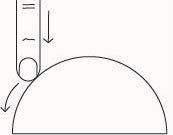
\includegraphics[scale=1]{images/curvatureillustration}
\caption{Illustration of a finger slipping off a curved surface.}
\label{fig:curvatureillustration}
\end{figure}
Beside that we found that the low resolution of 14 by 14 makes it hard for the 1\$ recognizer is not optimally detect a large set of gestures reliably. Curvature seems to have the only significant impact on overall performance which makes the thigh best suited additional to the fact that both participants prefer jeans fabric for interacting with the sensor. Although both participants liked operating the sensor, both agree that it gets unpleasant over time and it would be rather suited for occasional use. This is the result of the amount of force needed for a touch and the resulting strain in the operating finger. This varies for different body densities. Effects of abrupt changes in density (e.g. bone $\rightarrow$ muscle) were not yet investigated.

\section{Future work}
\label{summaryandfuturework.futurework}
\index{future work|}
Since the results of the hardware evaluation have shown that our technique of building a 2D textile touchpad is promising, the most immediate step would  be making the sensor actually wearable by integrating it into everyday clothing. This yields new challenges beside recognizing 2D touch. The wiring of sensor and microcontroller and the power supply should be imperceptible, lightweight, and compact. Furthermore the data processing and gesture recognition should be ported to the microcontroller. 
\\ \\
With a longitudinal evaluation of the system by wearing it for a period of several days we will be able to evaluate the wearability of the system and get insight in which conditions the noise increase and gesture recognition rate decrease.
\\ \\
Also increasing the resolution without making the surface larger could increase the reliability of gesture recognition. To increase the resolution we will try to decrease the spacing between the conductive lines and the width of the conductive threads. The lack of feedback is another issue for wearable devices. \cite{6636291} investigated this problem by providing haptic feedback. Getting feedback when acting close to the edge of the sensor area could greatly improve the performance. 
\index{future work|)}
\\ \\
Finally a number of embedded prototypes will be built with a larger range of fabrics used in today's clothes. Furthermore we will test different spacing techniques to improve wearability and decrease the required pressure. 
